This chapter reports the measured transfer. Section 4.1 gives the headline accuracy and how it varies across the city, answering the first half of RQ1. Sections 4.2 to 4.4 decompose the error and test the building and road subtractions, answering RQ2. Section 4.5 returns to spatial variation and shows the apparent location effect to be confounded. Section 4.6 reports the sampled corrections and what the reference data itself is worth. Section 4.7 answers RQ3 within the reliability the preceding sections establish.

\hypertarget{overall-accuracy-and-its-spatial-variation}{%
\section{Overall accuracy and its spatial variation}\label{overall-accuracy-and-its-spatial-variation}}

Against 3.2597 km² of labelled surface parking, the model predicts 4.8785 km² --- 1.50 times the labelled area.

\begin{table}[htbp]
\centering
\caption{Accuracy of the post-processed output over the 100 km² study area.}\label{tab:4.1}
\begin{adjustbox}{max width=\textwidth}
\begin{tabular}{@{}lrrr@{}}
\toprule
Aggregation & Precision & Recall & IoU \\
\midrule
\textbf{Micro, all confidence levels} & \textbf{0.5708} & \textbf{0.8543} & \textbf{0.5202} \\
Micro, confidence 2--3 only & 0.5287 & 0.8658 & 0.4886 \\
Macro (mean of 100 cells) & 0.5136 & 0.8468 & 0.4697 \\
\bottomrule
\end{tabular}
\end{adjustbox}
\end{table}
\restoreparskip

The pattern is asymmetric. Recall of 0.854 means the model finds most labelled parking; precision of 0.571 means that a little under half of what it returns is not labelled parking. Decomposed by area, TP is 2.7848 km², FP 2.0937 km² and FN 0.4749 km², the last being 14.6\% of labelled area.

\begin{figure}[htbp]
\centering
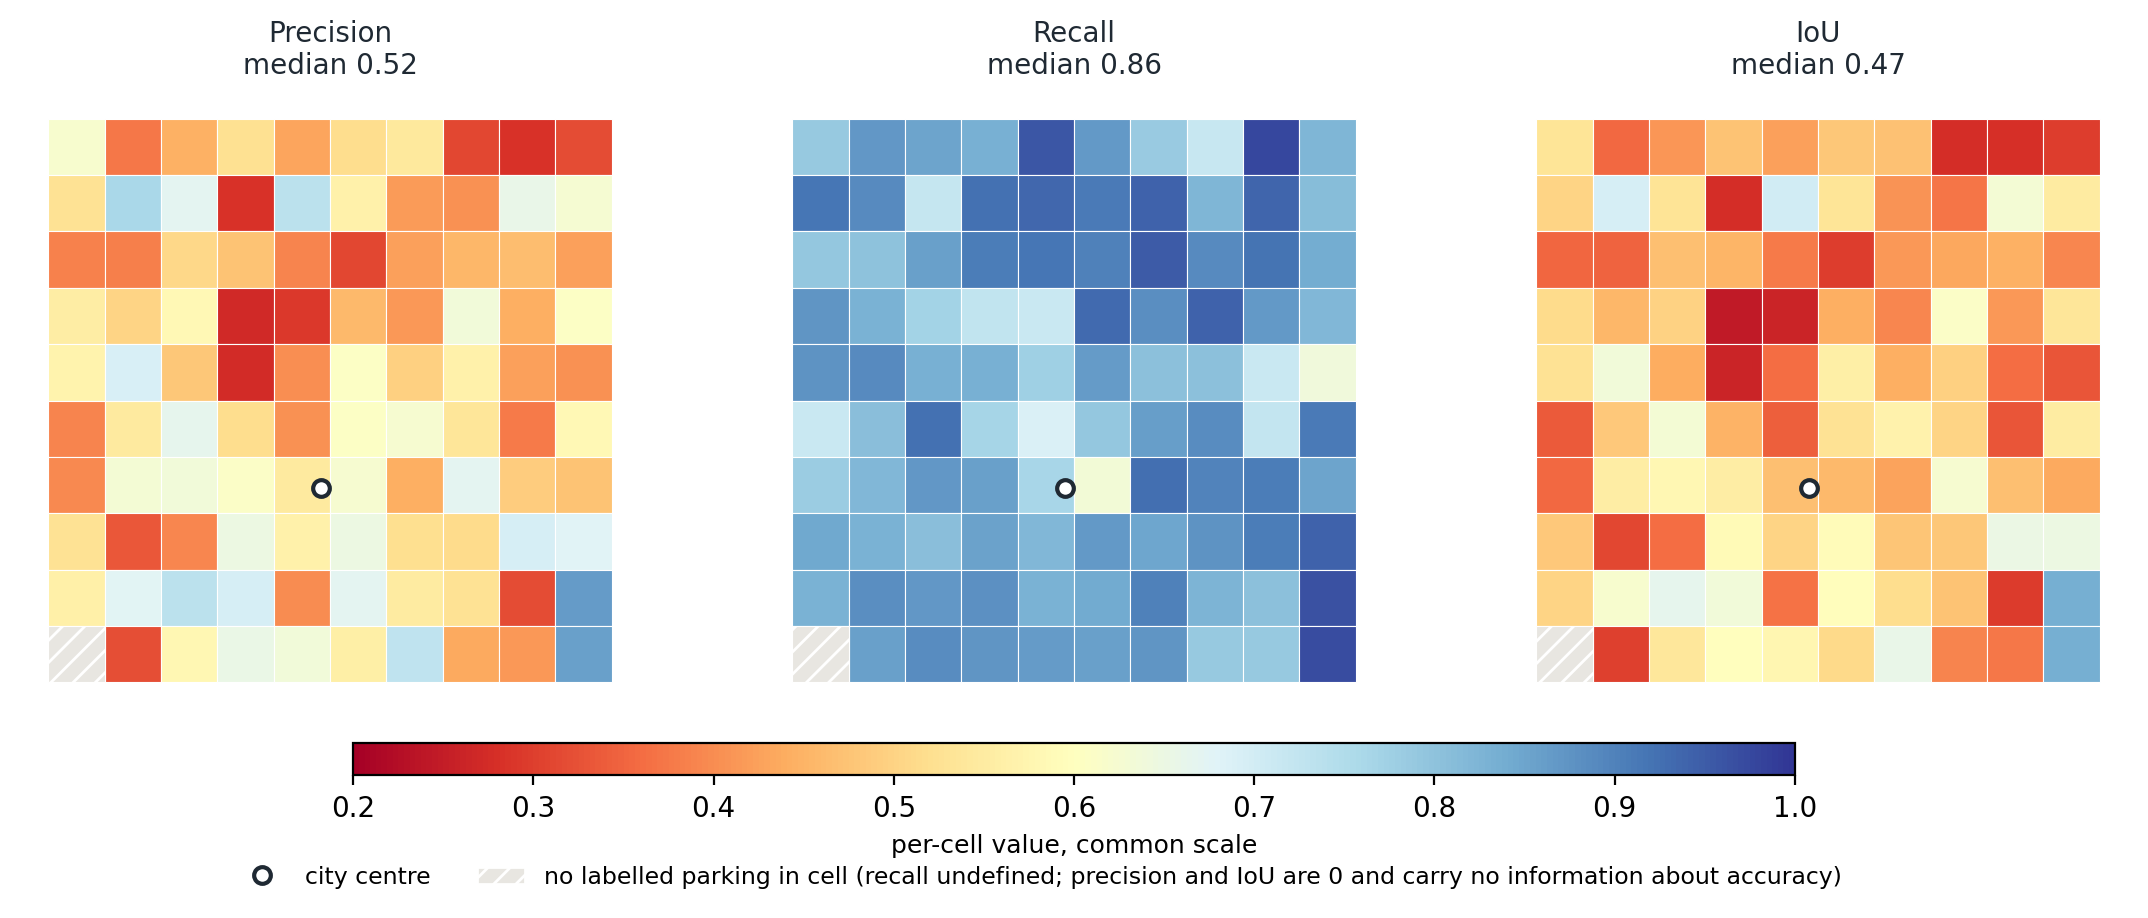
\includegraphics[width=\linewidth,height=0.82\textheight,keepaspectratio]{figures/fig_accuracy_maps.png}
\caption{Precision, recall and IoU for each 1 km² cell, on a common colour scale. Recall is generally high and less spatially variable than precision. One cell contains no labelled parking and is hatched.}
\label{fig:4.1}
\end{figure}\restoreparskip

Figure 4.1 shows that the asymmetry is not an artefact of aggregation: recall is generally high and varies less across the study area, while precision ranges from below 0.3 to above 0.8 between neighbouring cells. The macro figures fall below the micro figures on all three measures --- precision 0.514 against 0.571 --- indicating that cells contributing little parking area perform worse than the area-weighted total suggests.

Restricting the reference to the more confident labels does not improve precision; it lowers it, from 0.571 to 0.529. Since removing labels can only convert true positives into false positives, this establishes that the confidence-1 labels are not a substantial source of the measured over-prediction.

\hypertarget{false-positives}{%
\section{False positives}\label{false-positives}}

False-positive area is 2.0937 km². Figure 4.2 shows what it is made of.

\begin{figure}[htbp]
\centering
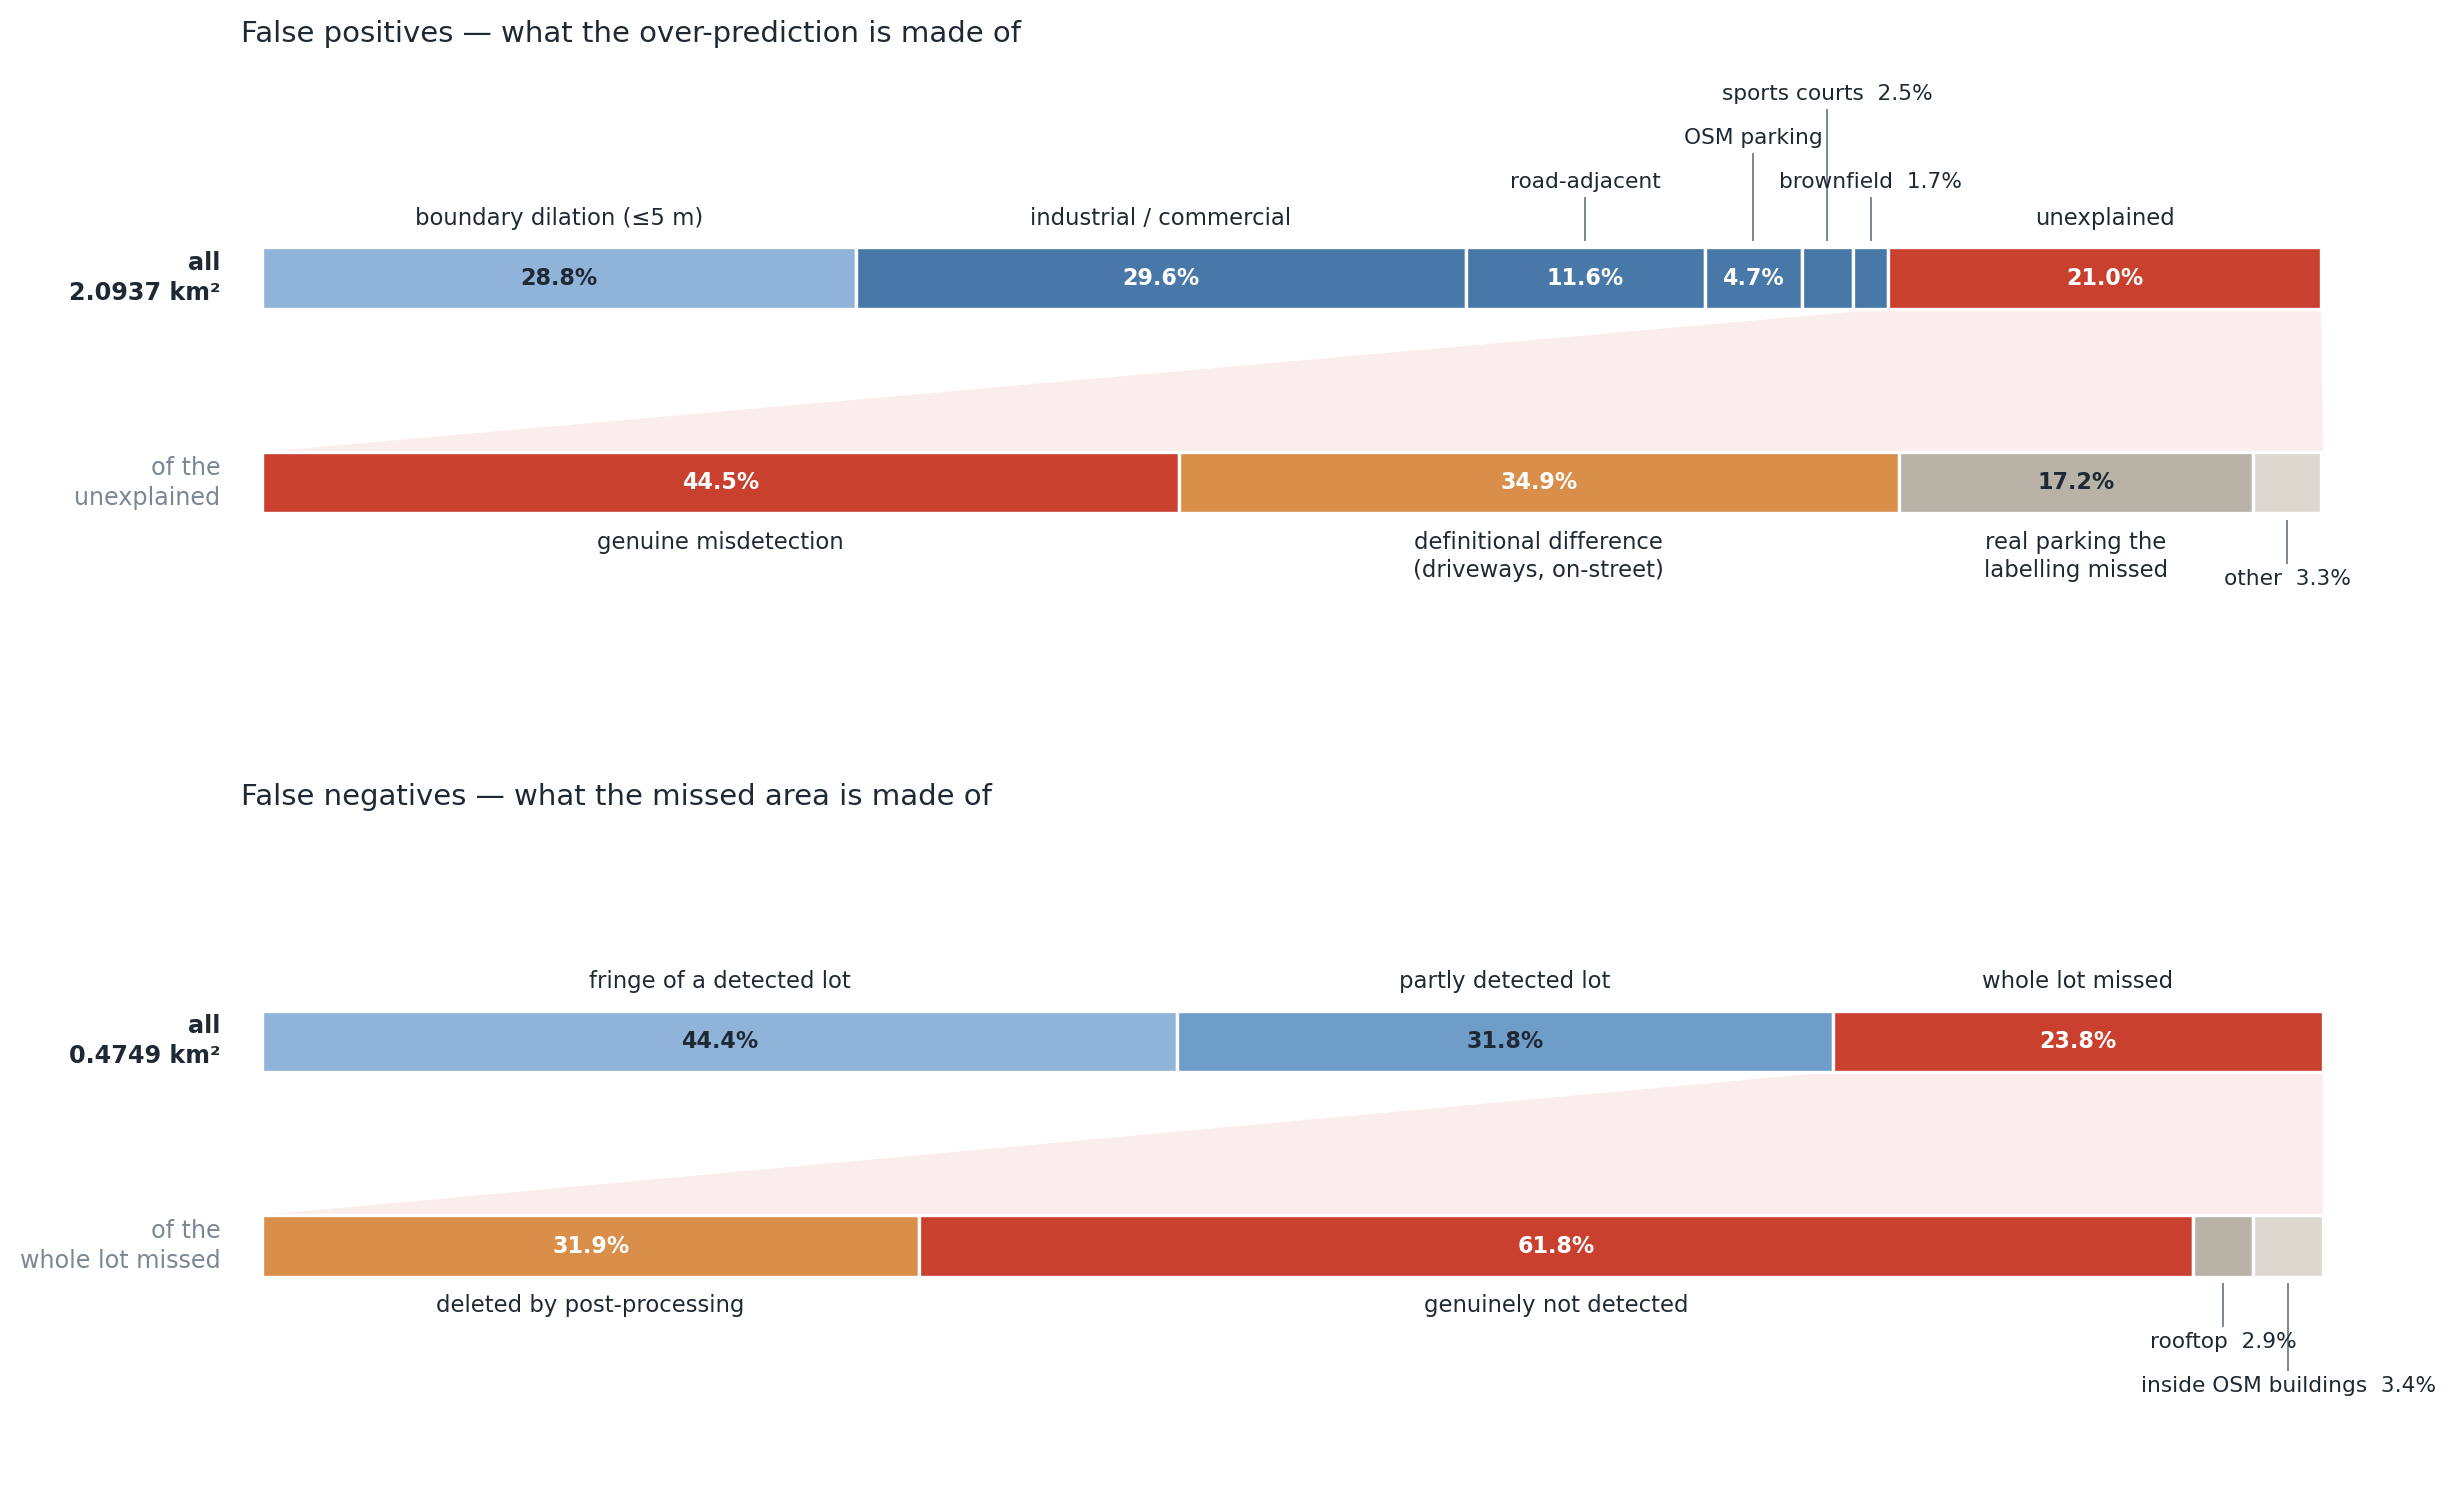
\includegraphics[width=\linewidth,height=0.82\textheight,keepaspectratio]{figures/fig_error_composition.png}
\caption{Composition of false-positive area (upper) and false-negative area (lower). In each case the lower bar expands the residual segment of the bar above it. Exclusive shares are of all FP or FN and sum to 100\%.}
\label{fig:4.2}
\end{figure}\restoreparskip

\textbf{Boundary effects account for a substantial minority.} False-positive area lying within a fixed distance of a labelled car park --- the model finding the right lot and drawing it too large --- is 17.3\% at 2 m, 28.8\% at 5 m and 36.3\% at 10 m. The three thresholds are reported because 5 m is a working convention; the value chosen shifts this component by nearly twenty percentage points.

\textbf{Attribution of the standalone remainder.} Table 4.2 gives the exclusive partition alongside the unordered diagnostic.

\begin{table}[htbp]
\centering
\caption{Where false-positive area falls. The two columns have different denominators and are not differences of one another: exclusive shares are assigned once each and sum to 100\%, while unordered overlaps are measured against all FP independently and may overlap one another.}\label{tab:4.2}
\begin{adjustbox}{max width=\textwidth}
\begin{tabular}{@{}lrr@{}}
\toprule
Layer & Exclusive (\% of all FP) & Unordered overlap (\% of all FP) \\
\midrule
Boundary dilation (≤ 5 m) & 28.8 & --- \\
Industrial / commercial land & 29.6 & \textbf{52.8} \\
Road-adjacent (+6 m) & 11.6 & 16.9 \\
OSM parking & 4.7 & 9.1 \\
Sports courts & 2.5 & 3.1 \\
Brownfield & 1.7 & 2.3 \\
Buildings & 0.0 & 0.0 \\
\textbf{Unexplained} & \textbf{21.0} & --- \\
\bottomrule
\end{tabular}
\end{adjustbox}
\end{table}
\restoreparskip

Industrial and commercial land coincides with over half of all false-positive area. Buildings account for none, because OSM building footprints have already been subtracted at the post-processing stage; false positives on buildings the OSM data does not record fall into the unexplained residual. Moving industrial land from an early position in the peeling order to last changes its exclusive share from 30.0\% to 29.6\%, so the attribution is not an artefact of the ordering.

\textbf{The unexplained residual divides into three unlike things.} Stratified sampling of 70 chips (Figure 4.3) estimates that 44.5\% of the residual is genuine misdetection --- grey hardstanding, goods yards, sports courts, unpaved ground and unmapped houses --- while 34.9\% is real parking that the annotation rules deliberately exclude, principally private driveways (20.2\%) and on-street parking (14.7\%). A further 17.2\% is parking the labelling itself missed. Percentages are of the sampling frame defined in §3.6.

\hypertarget{false-negatives}{%
\section{False negatives}\label{false-negatives}}

Missed area is 0.4749 km², 14.6\% of labelled parking. Measured against the prediction, 33.4\% of it lies within 2 m of something the model did find, 54.1\% within 5 m and 69.4\% within 10 m.

\textbf{Most missed area is the edge of a car park the model found.} Classifying missed area by how much of its parent lot the model covered gives a more useful split than any distance threshold:

\begin{table}[htbp]
\centering
\caption{Missed area by the state of the car park it belongs to.}\label{tab:4.3}
\begin{adjustbox}{max width=\textwidth}
\begin{tabular}{@{}llrrr@{}}
\toprule
Class & Coverage of the lot & Lots & Missed area (km²) & Share of FN \\
\midrule
Fringe of a well-detected lot & \textgreater{} 70\% & 1,638 & 0.2108 & 44.4\% \\
Partly detected & 10--70\% & 278 & 0.1510 & 31.8\% \\
\textbf{Whole lot missed} & ≤ 10\% & \textbf{121} & \textbf{0.1131} & \textbf{23.8\%} \\
\bottomrule
\end{tabular}
\end{adjustbox}
\end{table}
\restoreparskip

Nearly half of all missed area belongs to lots the model detected to better than 70\%. Only the third row is a detection failure in any useful sense, and it is not what it appears: 31.9\% of it was found by the model and then deleted by post-processing, with a further 2.9\% labelled as rooftop and 3.4\% falling inside OSM building footprints. After these automated attributions, 0.0699 km² remains unresolved, or 2.1\% of labelled area. The separate sampled assessment in §4.6 shows that reference--imagery disagreement also contributes to the whole-lot-miss population.

\textbf{Detection tracks size and annotator confidence.}

\begin{table}[htbp]
\centering
\caption{Detection rate by lot size and by labelling confidence.}\label{tab:4.4}
\begin{adjustbox}{max width=\textwidth}
\begin{tabular}{@{}lrrr@{}}
\toprule
Lot size & Lots & Mean detection rate & Missed entirely \\
\midrule
\textless{} 200 m² & 47 & 0.658 & \textbf{19.1\%} \\
200--500 m² & 563 & 0.763 & 8.2\% \\
500--1,000 m² & 573 & 0.805 & 5.4\% \\
1,000--2,500 m² & 559 & 0.852 & 3.0\% \\
2,500--5,000 m² & 182 & 0.850 & 4.9\% \\
\textgreater{} 5,000 m² & 113 & 0.864 & \textbf{1.8\%} \\
\bottomrule
\end{tabular}
\end{adjustbox}
\end{table}
\restoreparskip

\begin{table}[htbp]
\centering
\begin{adjustbox}{max width=\textwidth}
\begin{tabular}{@{}lrrr@{}}
\toprule
Confidence & Lots & Mean detection rate & Missed entirely \\
\midrule
1 (uncertain) & 435 & 0.713 & 10.6\% \\
2 & 1,137 & 0.829 & 3.8\% \\
3 (clear) & 465 & 0.856 & 5.4\% \\
\bottomrule
\end{tabular}
\end{adjustbox}
\end{table}
\restoreparskip

Lots below 200 m² are missed outright more than ten times as often as lots above 5,000 m². Detection is also lowest where the annotator was least certain, which indicates that part of the measured error reflects genuine ambiguity in the target rather than model deficiency.

\textbf{What the unresolved whole-lot population looks like.} Sampling of 42 chips estimates the composition of the residual as: not parking in the Digimap imagery 41.8\%, irregular layout 23.3\%, obscured by shadow or canopy 9.8\%, unusual surface 9.2\%, no cars present 6.3\%, vans and lorries rather than cars 5.2\%, and no markings 3.7\%.

\begin{figure}[htbp]
\centering
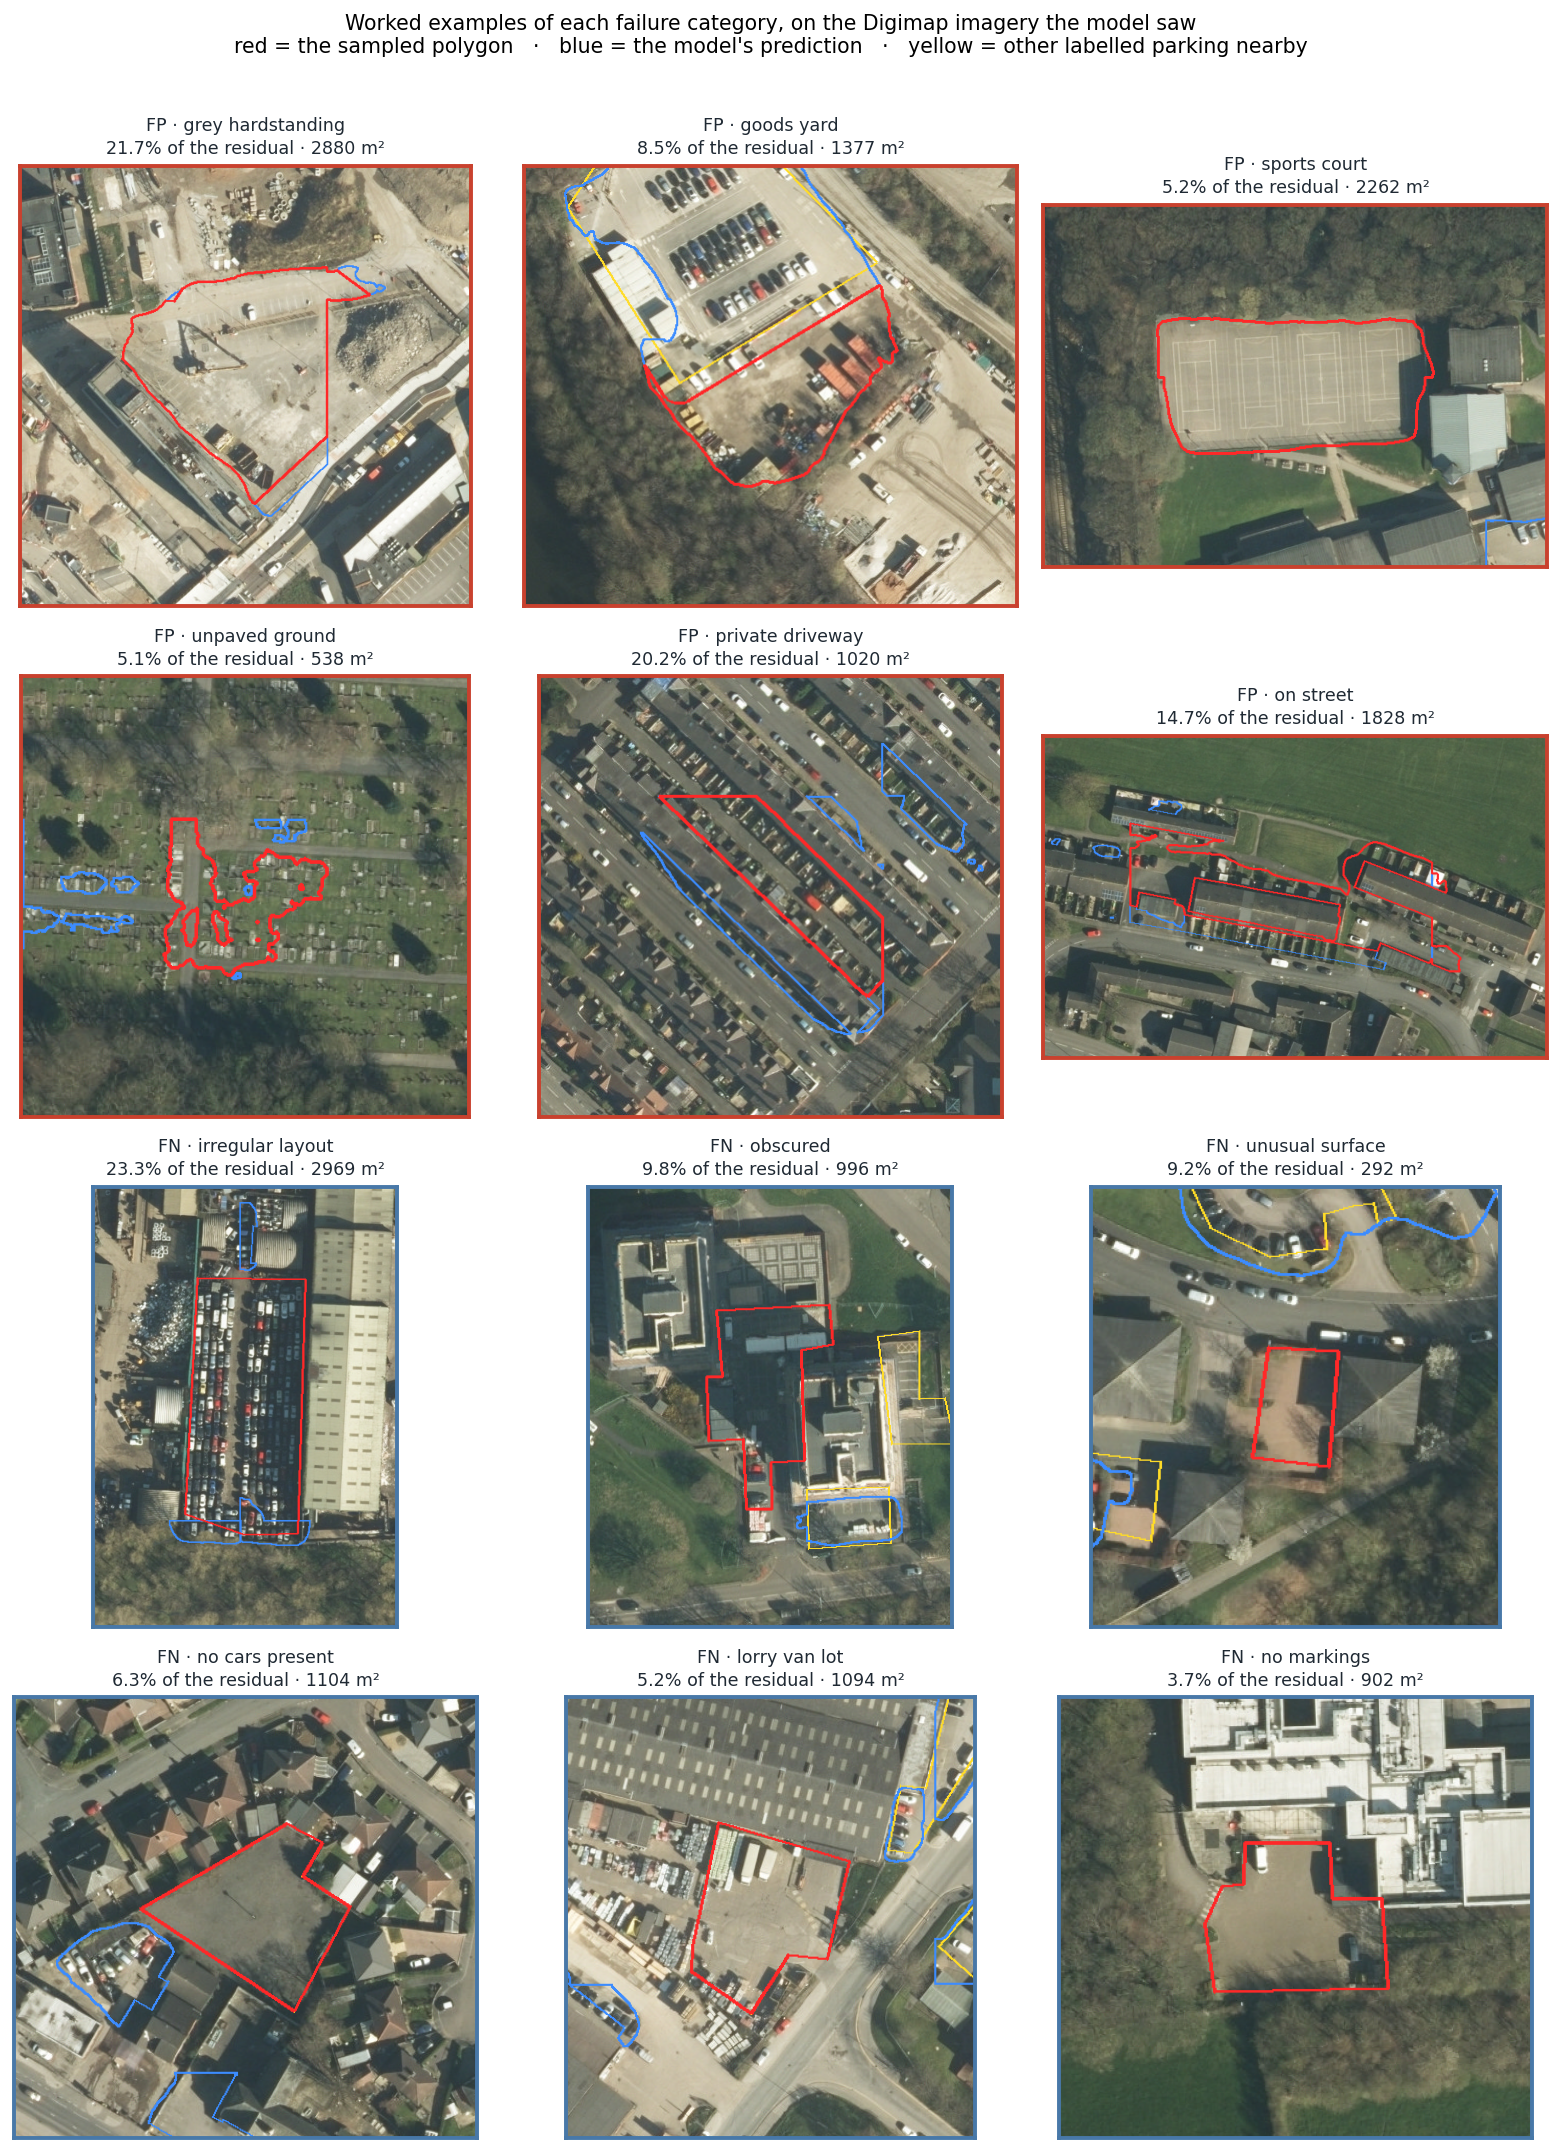
\includegraphics[width=\linewidth,height=0.82\textheight,keepaspectratio]{figures/fig_error_chips.png}
\caption{One worked example of each of twelve failure categories, on the Digimap imagery the model was given. Red outlines the sampled polygon, blue the model's prediction, yellow other labelled parking nearby.}
\label{fig:4.3}
\end{figure}\restoreparskip

Irregular layout was identified in 11 of 42 chips and absent markings in one. Although the resulting 3.7\% estimate for absent markings is imprecise, its interval remains well below that for irregular layout --- 3.7\% {[}0.6, 9.8{]} against 23.3\% {[}16.9, 31.1{]}. The evidence therefore supports the ordering, rather than a precise ratio: irregular arrangement was the most frequently identified mechanism and unmarked surfacing among the least, revising the expectation in §2.5 that unmarked surfaces would be the principal difficulty.

\hypertarget{post-processing-and-the-reference-layers-as-filters}{%
\section{Post-processing and the reference layers as filters}\label{post-processing-and-the-reference-layers-as-filters}}

\begin{figure}[htbp]
\centering
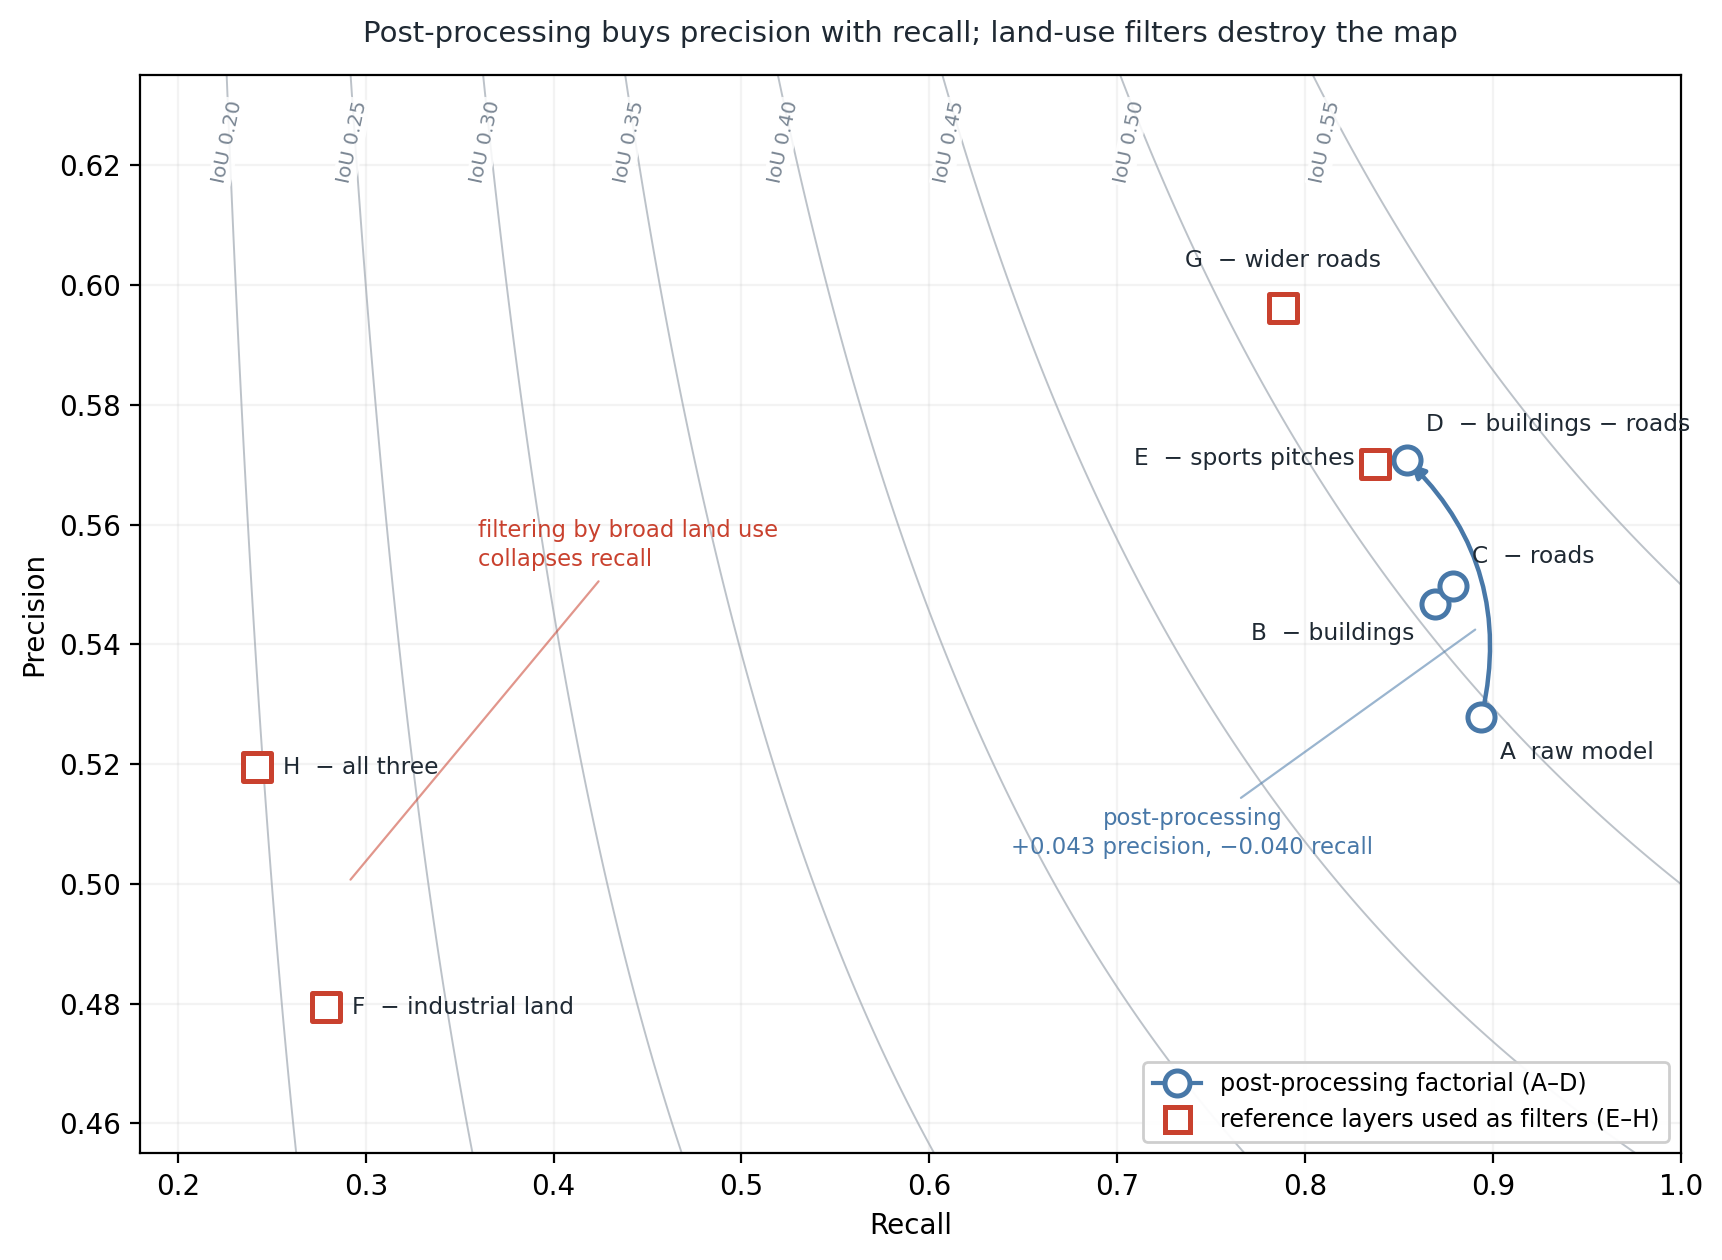
\includegraphics[width=\linewidth,height=0.82\textheight,keepaspectratio]{figures/fig_ablation.png}
\caption{The eight variants on the precision--recall plane, with IoU iso-lines. Circles are the building-and-road subtraction factorial; squares are reference layers applied as filters.}
\label{fig:4.4}
\end{figure}\restoreparskip

\begin{table}[htbp]
\centering
\caption{Ablation. Variants A--D vary the building and road subtractions; E--H apply further layers as filters to the finished map.}\label{tab:4.5}
\begin{adjustbox}{max width=\textwidth}
\begin{tabular}{@{}lrrr@{}}
\toprule
Variant & Precision & Recall & IoU \\
\midrule
A pre-subtraction output & 0.5278 & 0.8939 & 0.4967 \\
B − buildings & 0.5467 & 0.8691 & 0.5051 \\
C − roads & 0.5498 & 0.8789 & 0.5111 \\
\textbf{D − buildings − roads} & \textbf{0.5708} & \textbf{0.8543} & \textbf{0.5202} \\
E − sports pitches & 0.5701 & 0.8373 & 0.5132 \\
\textbf{F − industrial land} & 0.4794 & \textbf{0.2789} & \textbf{0.2140} \\
G − wider roads & \textbf{0.5962} & 0.7884 & 0.5140 \\
H − all three & 0.5195 & 0.2419 & 0.1976 \\
\bottomrule
\end{tabular}
\end{adjustbox}
\end{table}
\restoreparskip

Reconstructing D from the pre-subtraction output in a single operation reproduces the pipeline's own tile-by-tile result to within 0.0\% on all three measures, so the ablation isolates the two subtractions.

The two subtractions together raise precision by 0.043 and lower recall by 0.040, for a net IoU gain of 0.024. Each contributes roughly half. Applied as filters, the further layers behave quite differently. Subtracting industrial and commercial land --- the layer that coincided with 52.8\% of false-positive area --- collapses recall from 0.854 to 0.279 and IoU from 0.520 to 0.214, because supermarket and retail-park car parks sit on exactly that land. Widening the road buffers is the only variant to raise precision (to 0.596), and it still lowers IoU.

\textbf{The pipeline creates a blind spot of its own.} Sixteen labelled lots, 0.0395 km² or 1.21\% of the reference, are rooftop parking.

\begin{table}[htbp]
\centering
\caption{Rooftop parking, before and after post-processing.}\label{tab:4.6}
\begin{adjustbox}{max width=\textwidth}
\begin{tabular}{@{}lr@{}}
\toprule
Measure & Value \\
\midrule
Recall on rooftop lots, before subtraction & \textbf{0.916} \\
Recall on rooftop lots, after subtraction & \textbf{0.115} \\
Recall on non-rooftop lots, before subtraction & 0.894 \\
Rooftop area falling inside OSM buildings & 85.6\% \\
Rooftop area detected then removed & \textbf{80.1\%} \\
\bottomrule
\end{tabular}
\end{adjustbox}
\end{table}
\restoreparskip

The pre-subtraction output detects rooftop parking slightly \emph{better} than ground-level parking. Subtracting building footprints removes four fifths of it.

\hypertarget{accuracy-and-location}{%
\section{Accuracy and location}\label{accuracy-and-location}}

\begin{table}[htbp]
\centering
\caption{Correlations with per-cell precision, recall and IoU (Pearson r, p in brackets). Recall statistics use the 99 cells with labelled parking.}\label{tab:4.7}
\begin{adjustbox}{max width=\textwidth}
\begin{tabular}{@{}lrrrr@{}}
\toprule
Metric & Distance & Parking share & Distance \textbar{} parking share & Parking share \textbar{} distance \\
\midrule
\textbf{Precision} & −0.172 (0.087) & \textbf{+0.536 (\textless0.0001)} & +0.186 (0.065) & \textbf{+0.540 (\textless0.0001)} \\
Recall & +0.181 (0.073) & +0.103 (0.313) & +0.289 (0.004) & +0.250 (0.013) \\
IoU & −0.127 (0.208) & \textbf{+0.515 (\textless0.0001)} & +0.229 (0.022) & \textbf{+0.540 (\textless0.0001)} \\
\bottomrule
\end{tabular}
\end{adjustbox}
\end{table}
\restoreparskip

Distance from the city centre does not predict precision. The share of a cell given over to parking does, strongly, and continues to do so after controlling for distance. The reverse does not hold: controlling for parking share, the distance effect is not significant. Distance and parking share are themselves correlated at −0.562.

All three metrics are reported to avoid selective presentation, but only precision is interpreted here. The partial correlations for recall and IoU reach significance while their raw correlations do not, and their signs reverse between the two; with n = 100 and two strongly correlated predictors this pattern is not a stable basis for a claim.

Read across distance bands, precision falls from 0.584 within 1 km to 0.485 beyond 4 km while recall stays between 0.70 and 0.86 (see Figure 4.5 and Appendix B). The band means move with parking share, not with distance.

\begin{figure}[htbp]
\centering
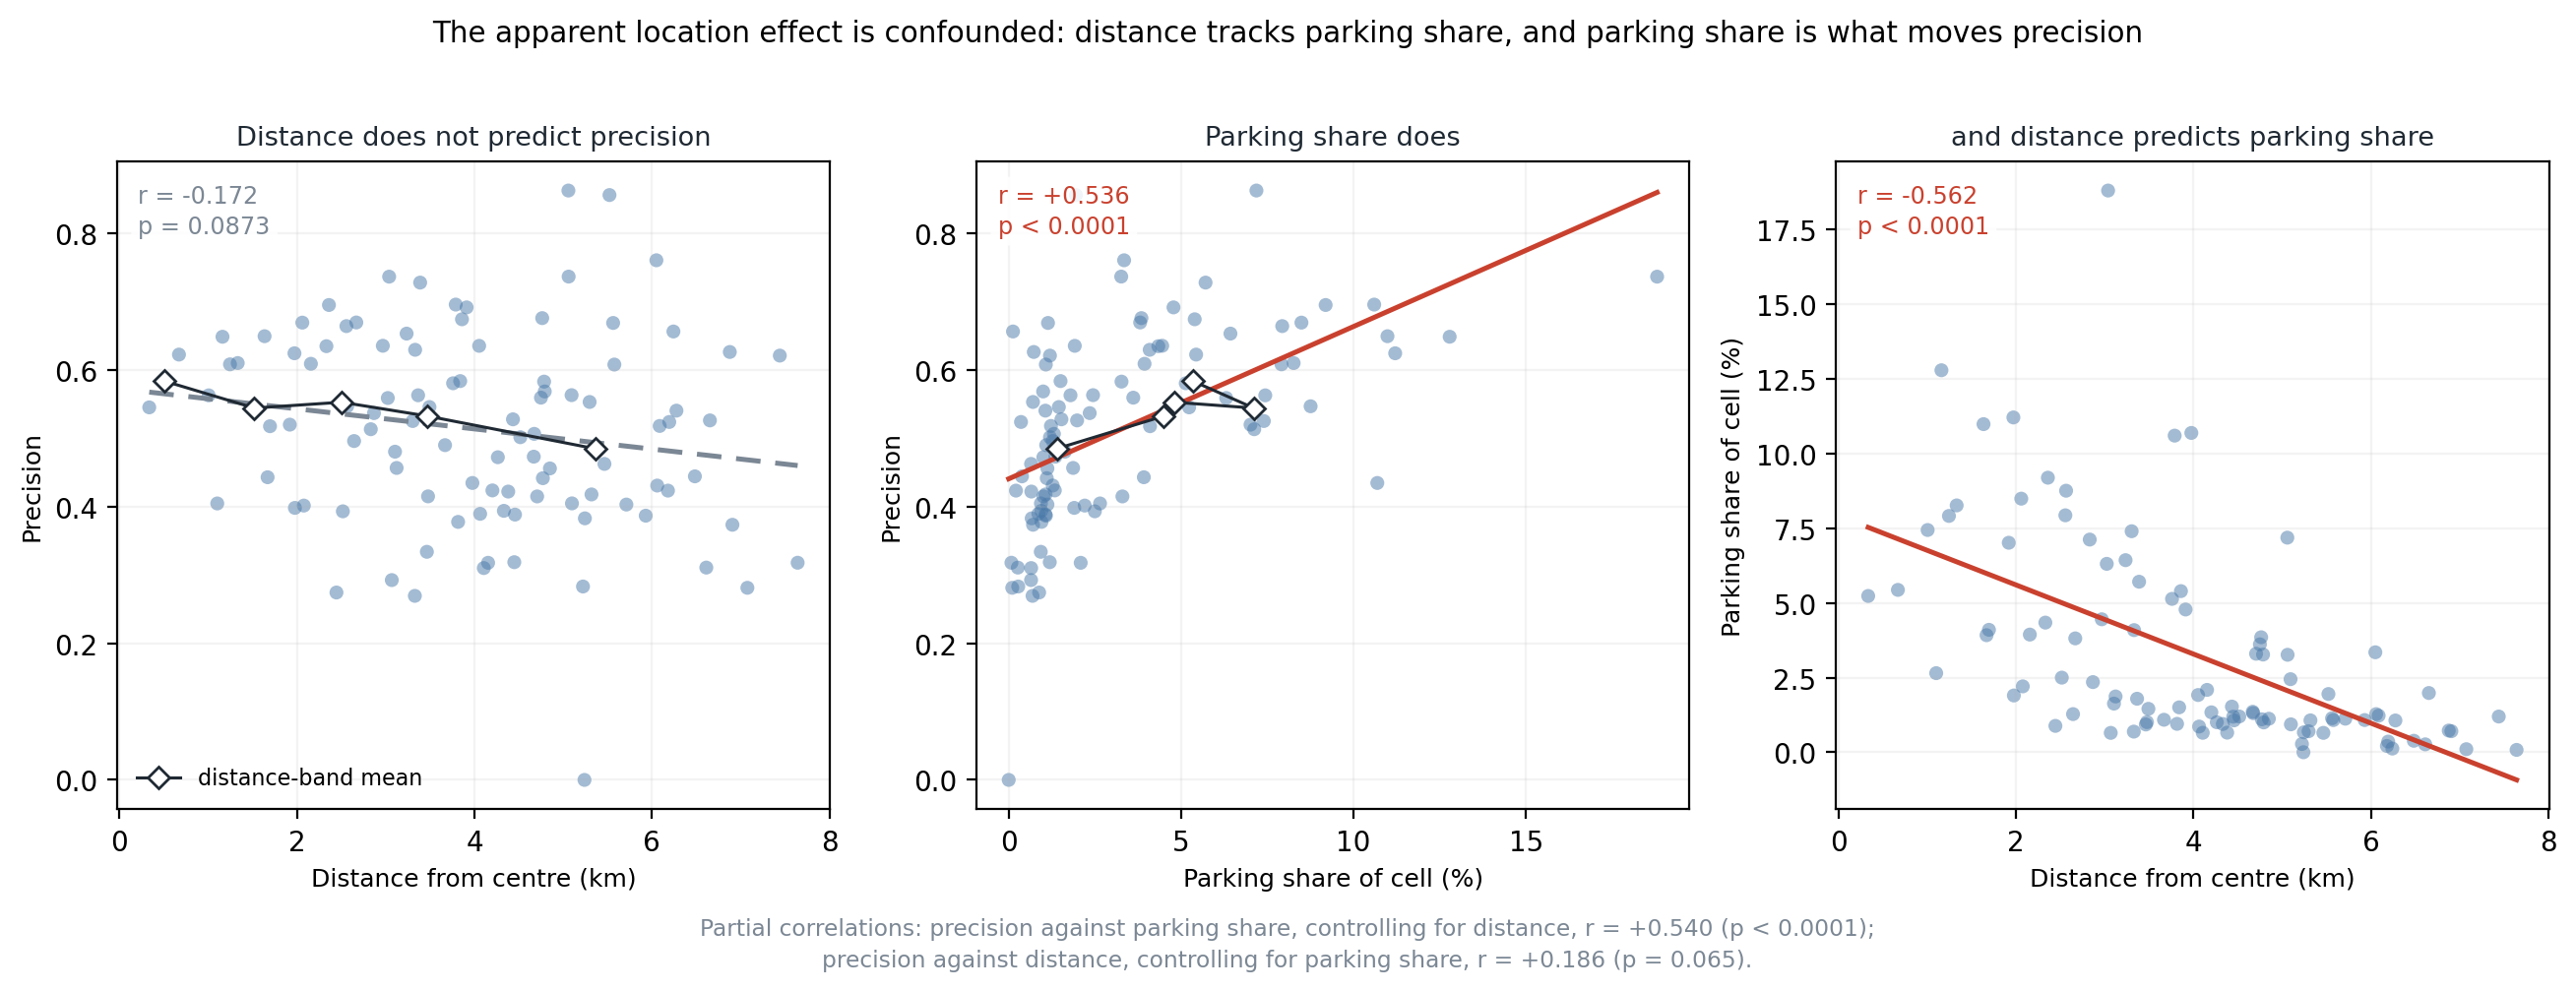
\includegraphics[width=\linewidth,height=0.82\textheight,keepaspectratio]{figures/fig_accuracy_vs_location.png}
\caption{Per-cell precision against distance and against parking share, and parking share against distance. Solid red fits are significant at p \textless{} 0.05; the dashed grey fit is not. Diamonds are distance-band means.}
\label{fig:4.5}
\end{figure}\restoreparskip

\hypertarget{sampled-corrections-and-what-the-reference-is-worth}{%
\section{Sampled corrections, and what the reference is worth}\label{sampled-corrections-and-what-the-reference-is-worth}}

Applying the sampled estimates as corrections gives four cumulative variants:

\begin{table}[htbp]
\centering
\caption{Accuracy under cumulative correction.}\label{tab:4.8}
\begin{adjustbox}{max width=\textwidth}
\begin{tabular}{@{}lrrrrr@{}}
\toprule
Variant & Reference (km²) & Prediction (km²) & Precision & Recall & IoU \\
\midrule
\textbf{1 As measured} & 3.2597 & 4.8785 & \textbf{0.5708} & \textbf{0.8543} & \textbf{0.5202} \\
2 + reference-side (−0.0313, not parking in the imagery) & 3.2284 & 4.8785 & 0.5708 & 0.8626 & 0.5233 \\
3 + prediction-side (+0.0667, parking the labelling missed) & 3.2951 & 4.8785 & 0.5845 & 0.8654 & 0.5358 \\
\textbf{4 Effective (−0.1358, definitional exclusions removed)} & 3.2951 & 4.7427 & \textbf{0.6012} & 0.8654 & \textbf{0.5498} \\
\bottomrule
\end{tabular}
\end{adjustbox}
\end{table}
\restoreparskip

Across the four variants, precision rises from 0.571 to 0.601, about half of the gain coming from the final removal of on-street parking and private driveways --- real parking excluded by the target definition rather than model error. Recall changes only from 0.854 to 0.865. For variant 4, the stratified bootstrap gives 95\% intervals of {[}0.5941, 0.6090{]} for precision, {[}0.8635, 0.8675{]} for recall and {[}0.5434, 0.5569{]} for IoU; its precision interval remains above the measured 0.5708. The headline pattern is therefore unchanged, and variant 1 remains the primary result.

\textbf{OpenStreetMap, assessed against the same reference.} OSM records 1.7641 km² of parking across 985 polygons, against 3.2597 km² across 2,037 labelled polygons. It overlaps only 1.1882 km², or 36.5\% of labelled parking, leaving 63.5\% absent from OSM. Similar median polygon areas (763 and 799 m²) suggest that this incompleteness is not explained simply by polygon size. Within the 0.2610 km² sampling frame of OSM parking polygons above 100 m² and no more than 10\% covered by the labels, 63.2\% is estimated to show no parking in the model-input imagery. The 11 sampled features in that category had a median last-edit year of 2025, so stale OSM records are not supported as a general explanation, subject to the timestamp limitation in §3.8.

\hypertarget{the-extent-and-distribution-of-surface-parking}{%
\section{The extent and distribution of surface parking}\label{the-extent-and-distribution-of-surface-parking}}

\begin{table}[htbp]
\centering
\caption{Surface parking as a share of land, by distance band.}\label{tab:4.9}
\begin{adjustbox}{max width=\textwidth}
\begin{tabular}{@{}lrrrr@{}}
\toprule
Band & Cells & Labelled & Model & Calibrated (km²) \\
\midrule
\textless{} 1 km & 2 & 5.33\% & 6.42\% & 0.086 \\
\textbf{1--2 km} & 11 & \textbf{7.11\%} & 10.35\% & 0.761 \\
2--3 km & 14 & 4.80\% & 7.19\% & 0.673 \\
3--4 km & 22 & 4.50\% & 6.53\% & 0.959 \\
\textgreater{} 4 km & 51 & 1.39\% & 2.29\% & 0.781 \\
\textbf{Whole area} & 100 & \textbf{3.26\%} & 4.88\% & 3.2595 \\
\bottomrule
\end{tabular}
\end{adjustbox}
\end{table}
\restoreparskip

The calibrated column applies the whole-area factor from §3.9. Its whole-area value is an identity; the band rows show residuals when that citywide factor is applied within each band (−19.6\% to +10.0\%), not an independent transfer test.

The complete-coverage reference contains 3.2597 km² of surface parking, or 3.26\% of the 100 km² study area. The sampled reference corrections in §4.6 raise this to 3.2951 km² (3.30\%), a shift of less than 0.1 percentage points.

Parking share peaks at 7.11\% in the 1--2 km band and then falls monotonically to 1.39\% beyond 4 km. The apparent central dip to 5.33\% is uncertain because the \textless1 km band contains only two cells. Across cells, the distribution is strongly right-skewed: mean 3.26\%, median 1.71\%, maximum 18.81\%, with six cells above 10\%.

\begin{figure}[htbp]
\centering

\includegraphics[width=\linewidth,height=0.82\textheight,keepaspectratio]{figures/parking_extent.png}
\caption{Labelled parking share by cell (white circle: City Square), labelled and predicted shares against distance, and the distribution of labelled shares across the 100 cells.}
\label{fig:4.6}
\end{figure}\restoreparskip

\textbf{Calibration and the grain at which it holds.} For a map with precision \emph{p} and recall \emph{r}, reference-equivalent area is estimated as predicted area × \emph{p}/\emph{r} (§3.9); here, 4.8785 × \emph{p}/\emph{r} = 3.2595 km². This is an identity on the cells used to fit the factor. Table 4.10 tests it on held-out cells.

\begin{table}[htbp]
\centering
\caption{Error of the calibrated estimate on cells excluded from fitting the factor.}\label{tab:4.10}
\begin{adjustbox}{max width=\textwidth}
\begin{tabular}{@{}llrrrr@{}}
\toprule
Scheme & Held out & Tests & Mean error & 5th--95th pct. & Within ±25\% \\
\midrule
\textbf{Random half split} & 50 cells & 200 & +0.3\% & \textbf{−6.6\% to +7.8\%} & 100\% \\
Leave one distance band out & 1 band & 5 & −2.9\% & −16.9\% to +10.6\% & --- \\
\textbf{Leave one cell out} & 1 cell & 99 & +16.5\% & −22.0\% to +80.5\% & \textbf{63\%} \\
\bottomrule
\end{tabular}
\end{adjustbox}
\end{table}
\restoreparskip

Across the 200 random half splits, the central 90\% of held-out errors runs from −6.6\% to +7.8\%, showing that a factor fitted on half the city transfers to a comparable sub-area within the same city. This is not an uncertainty interval for the directly labelled 3.26\%. At 1 km², the estimator becomes unstable: only 63\% of cells fall within ±25\%, and the +16.5\% mean is inflated by small denominators (median absolute error 0.0035 km² against mean labelled area 0.0329 km²).

\begin{figure}[htbp]
\centering

\includegraphics[width=\linewidth,height=0.82\textheight,keepaspectratio]{figures/calibration_transfer.png}
\caption{Held-out calibration errors under the three schemes. Red lines mark medians and dashed black lines means; the distance-band panel contains only five tests.}
\label{fig:4.7}
\end{figure}\restoreparskip
